\documentclass[twocolumn]{aastex61}
%\documentclass{emulateapj}
%\usepackage[colorlinks,urlcolor=blue,citecolor=blue,linkcolor=blue]{hyperref} 
\usepackage{graphicx,natbib}
\citestyle{aa}
\usepackage[space]{grffile}
\usepackage{latexsym}
\usepackage{amsfonts,amsmath,amssymb}
\usepackage{url}
\usepackage[utf8]{inputenc}
\usepackage{fancyref}
\usepackage{hyperref}
\usepackage{multirow}
\hypersetup{colorlinks=false,pdfborder={0 0 0},}

\newcommand{\rf}{\emph{realfast}}
\newcommand{\frb}{FRB 121102}

\begin{document}

\title{\frb: Multi-Telescope Burst Properties and Implications for FRB Population}
\shorttitle{\frb\ Burst Properties}
\shortauthors{Law et al.}

\author[0000-0002-4119-9963]{C.~J.~Law}
\affiliation{Dept of Astronomy and Radio Astronomy Lab, University of California, Berkeley, CA 94720, USA}

%\author{M.~W.~Abruzzo}
%\affiliation{Haverford College, 370 Lancaster Ave, Haverford, PA 19041, USA}

%\author{C.~G.~Bassa}
%\affiliation{ASTRON, Netherlands Institute for Radio Astronomy, Postbus 2, 7990 AA, Dwingeloo, The Netherlands}

%\author{S.~Bogdanov}
%\affiliation{Columbia Astrophysics Laboratory, Columbia University,  New York, NY 10027, USA}

\author{G.~C.~Bower}
\affiliation{Academia Sinica Institute of Astronomy and Astrophysics, 645 N. A'ohoku Place, Hilo, HI 96720, USA}

\author{S.~Burke-Spolaor}
\affiliation{National Radio Astronomy Observatory, Socorro, NM 87801, USA}
\affiliation{Department of Physics and Astronomy, West Virginia University, Morgantown, WV 26506, USA}
\affiliation{Center for Gravitational Waves and Cosmology, West Virginia University, Chestnut Ridge Research Building, Morgantown, WV 26505}

\author{B.~J.~Butler}
\affiliation{National Radio Astronomy Observatory, Socorro, NM 87801, USA}
\author{S.~Chatterjee}
\affiliation{Cornell Center for Astrophysics and Planetary Science and Department of Astronomy, Cornell University, Ithaca, NY 14853, USA}

\author{J.~M.~Cordes}
\affiliation{Cornell Center for Astrophysics and Planetary Science and Department of Astronomy, Cornell University, Ithaca, NY 14853, USA}

\author{P.~Demorest}
\affiliation{National Radio Astronomy Observatory, Socorro, NM 87801, USA}

\author{J.~W.~T.~Hessels}
\affiliation{ASTRON, Netherlands Institute for Radio Astronomy, Postbus 2, 7990 AA, Dwingeloo, The Netherlands}
\affiliation{Anton Pannekoek Institute for Astronomy, University of Amsterdam, Science Park 904, 1098 XH Amsterdam, The Netherlands}

\author{R.~Fender}
\affiliation{University of Oxford, UK}

%\author{V.~M.~Kaspi}
%\affiliation{Department of Physics and McGill Space Institute, McGill University, 3600 University St., Montreal, QC H3A 2T8, Canada}

%\author{A.~Keimpema}
%\affiliation{Joint Institute for VLBI ERIC, Postbus 2, 7990 AA Dwingeloo, The Netherlands}

%\author{H.~J.~van~Langevelde}
%\affiliation{Joint Institute for VLBI ERIC, Postbus 2, 7990 AA Dwingeloo, The Netherlands}
%\affiliation{Sterrewacht Leiden, Leiden University, Postbus 9513, 2300 RA, Leiden, the Netherlands}

\author{T.~J.~W.~Lazio}
\affiliation{Jet Propulsion Laboratory, California Institute of Technology, Pasadena, CA 91109, USA}

%\author[0000-0001-9814-2354]{B.~Marcote}
%\affiliation{Joint Institute for VLBI ERIC, Postbus 2, 7990 AA Dwingeloo, The Netherlands}

\author{M.~A.~McLaughlin}
\affiliation{Department of Physics and Astronomy, West Virginia University, Morgantown, WV 26506, USA}
\affiliation{Center for Gravitational Waves and Cosmology, West Virginia University, Chestnut Ridge Research Building, Morgantown, WV 26505}

\author{K.~Mooley}
\affiliation{University of Oxford, UK}

%\author{Z.~Paragi}
%\affiliation{Joint Institute for VLBI ERIC, Postbus 2, 7990 AA Dwingeloo, The Netherlands}

%\author{S.~M.~Ransom}
%\affiliation{National Radio Astronomy Observatory, Charlottesville, VA 22903, USA}

\author{M.~Rupen}
\affiliation{National Research Council of Canada, Herzberg Astronomy and Astrophysics, Dominion Radio Astrophysical Observatory, P.O. Box 248, Penticton, BC V2A 6J9, Canada}

\author{L.~G.~Spitler}
\affiliation{Max-Planck-Institut f\"ur Radioastronomie, Auf dem H\"ugel 69, D-53121 Bonn, Germany}

\author{P.~Scholz}
\affiliation{National Research Council of Canada, Herzberg Astronomy and Astrophysics, Dominion Radio Astrophysical Observatory, P.O. Box 248, Penticton, BC V2A 6J9, Canada}

\author{A.~Seymour}
\affiliation{Arecibo Observatory, HC3 Box 53995, Arecibo, PR 00612, USA}
\affiliation{Max-Planck-Institut f\"ur Radioastronomie, Auf dem H\"ugel 69, Bonn, D-53121, Germany}

%\author{S.~P.~Tendulkar}
%\affiliation{Department of Physics and McGill Space Institute, McGill University, 3600 University St., Montreal, QC H3A 2T8, Canada}

\author{R.~S.~Wharton}
\affiliation{Cornell Center for Astrophysics and Planetary Science and Department of Astronomy, Cornell University, Ithaca, NY 14853, USA}


\begin{abstract}
The millisecond radio transients known as Fast Radio Bursts have recently emerged as a mysterious, new class of astrophysical transient. The discovery of repeating bursts from \frb\ has shown that at least some FRBs are not cataclysmic and opened potential for studying FRB properties via a homogenous sample of bursts. The recent localization of \frb\ with the Very Large Array has helped measure its distance and a host of intrinsic properties. This localization was made with 9 bursts seen by the VLA in coordination the Arecibo, Effelsberg, and AMI-LA observatories. We present a detailed analysis of these bursts, including the first simultaneous detection of an FRB with multiple telescopes. We show that the burst spectra typically have a broad Gaussian shape on the scale of $\sim500$~MHz with fine spectral structure consistent with either scintillation or unresolved temporal structure. We present the luminosity distribution and temporal statistics for \frb\ and argue that the whole FRB population is adequately described by a single class similar to \frb. We close with thoughts on optimal strategies to make new interferometric localizations of FRBs.
\end{abstract}

\section{Introduction}
Fast Radio Bursts (FRBs) are a new class of millisecond-duration radio transient with a dispersion measure (DM) that implies that they originate outside of our Galaxy. At extragalactic (and potentially cosmological) distances, they are not only unusually luminous, but they provide a new tracer of other galaxies and the intergalactic medium (IGM). In this way, FRBs have opened a whole new playground in astrophysics \citep[e.g.,][]{2014A&A...562A.137F, 2014ApJ...780L..33M, 2016MNRAS.457..232C}. However, that potential has been hamstrung by the lack of a definitive association of an FRB to an extragalactic host.

This paper is part of a series that presents the first localization and unambiguous identification of an FRB host (CITE: LOC, OPT, EVN, RADIO CPART, XRAY, EFF, WEIRD). \frb, also known as the ``repeating FRB'', was first detected in November 2012 by the Arecibo Observatory \citep{2014ApJ...790..101S}. In mid 2015, new Arecibo observations revealed a series of bursts at the same DM and sky position demonstrating that FRBs are capable of repetition \citep{2016Natur.531..202S}. Beginning in August of 2015, we made the first of nine detections of \frb\ with the Very Large Array (CITE: LOC) and localized it with a precision of 0.1\arcsec. Deep radio and optical observing shows that \frb\ is unambiguously associated with a persistent radio and optical source at a redshift of 0.193 (CITE: OPT, EVN).

\frb\ has now been localized three orders of magnitude better than any other FRB and placed at a cosmological distance. Its lookback and luminosity distances are 746 and 972 Mpc \citep{planck15}, which are orders of magnitude larger than any other millisecond transient. This shows that FRBs are more luminous than any other millisecond radio transient, have a significant DM contribution from the IGM, and can be used to probe the IGM and their host galaxy. The promise implied by the first reported FRB \citep{2007Sci...318..777L} is now being realized.

The confirmation of a cosmological distance for \frb\ could have wide-ranging implications for the FRB population as a whole. However, it has not been demonstrated that \frb\ is representative of the overall FRB population. In fact, the repetition of its bursts is unique among all FRBs \citep{2015MNRAS.454..457P}, so it is natural to ask whether \frb\ is representative. An important first step is to demonstrate that the properties of \frb\ are consistent with the significant body of facts for the overall population \citep{2015MNRAS.451.3278M, 2016MPLA...3130013K}. The repeating nature of \frb\ provides us with several statistical tests we can use to test this connection.

We can also assume that \frb\ is representative and use it to constrain the physical processes at play in the overall FRB population. Although we now know that FRBs are luminous, it is not yet clear what process generates the radio bursts themselves \citep{2014PhRvD..89j3009K, 2014ApJ...785L..26L, 2016MNRAS.457..232C}. The simultaneous \frb\ observing campaign with the VLA, Arecibo, Effelsberg, GBT, and AMI-LA gives a more complete picture of the spectral structure of FRB radio emission. FRB repetition also has strong implications for the number of FRB-generating systems in the universe \citep{2016MNRAS.458L..89C}.

Given that FRBs are now known to be useful probes of the IGM, there is even more motivation to make new detections and localizations. The relatively faint counterpart to \frb\ argues that direct localization of the radio burst will continue to be the best way to find optical hosts to measure distances. Our multi-telescope constraints on burst spectra, measurement of host properties, burst rate estimates, and other properties will inform new strategies for finding FRBs.

\section{Observations}

\begin{figure*}[t]
\begin{center}
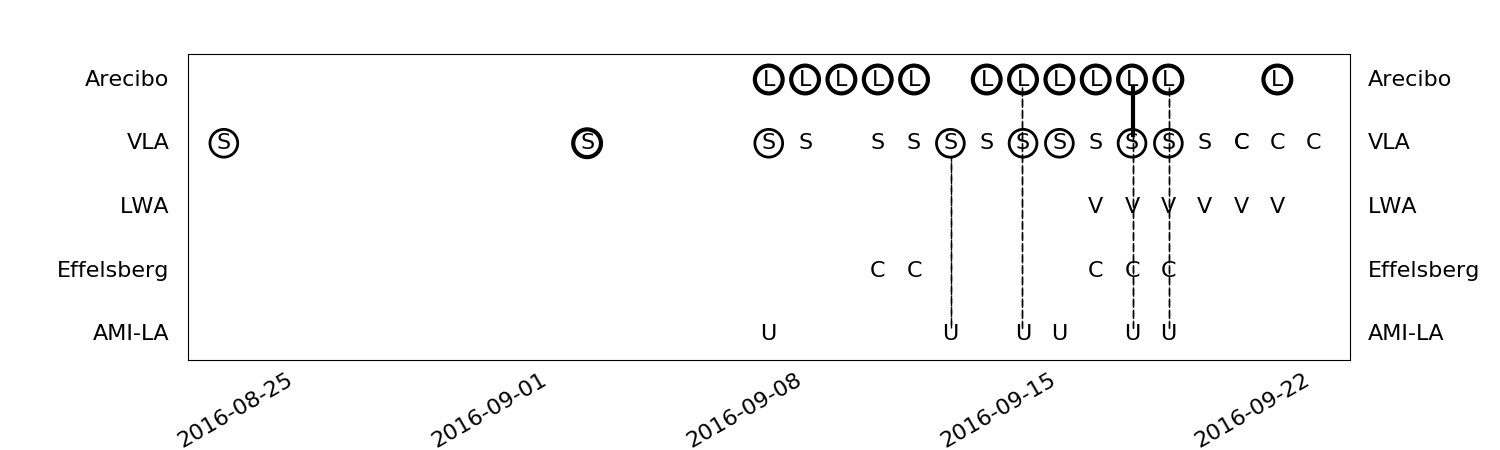
\includegraphics[width=2\columnwidth]{timeline}
\caption{Summary of observing coverage and detections of \frb\ during the multi-telescope observing campaign in August and September 2016. Symbols show days with observations and circles highlight observations that detected bursts from \frb. Multiple circles indicate multiple burst detections, except for Arecibo, which typically has multiple detections per observing session (a detailed analysis is left for a future paper). The black dashed lines show the VLA burst detections with simultaneous coverage at other telescopes. The solid black line shows the simultaneous burst detection at VLA and Arecibo.
\label{fig:multi}}
\end{center}
\end{figure*}

The data presented here were obtained from multiple programs and telescopes, but the central goal was to interferometrically localize \frb\ with the VLA. The observing strategy was to ensure simultaneous observing between the VLA and Arecibo observatories and add other observatories added on a best-effort basis. We coordinated observing between the VLA, Arecibo, Effelsberg, and AMI-LA telescopes, as shown in figure \ref{fig:multi}. Below, we summarize these observations, with a focus on those conducted simultaneous with VLA burst detections from \frb.

\subsection{VLA}
The \frb\ observing campaign started in late 2015 with a 10~hr campaign observed at 1.4~GHz in the compact D configuration. In April through May 2016, we conducted a 40~hr campaign at 3~GHz in the C and CnB configurations in coordination with Arecibo. We concluded with a new, 40~hr, coordinated campaign from August through September 2016 in the B configuration and during the move to the most extended A configuration. In this last campaign, the first 34 hours of VLA observations were made at 3~GHz, while the last 6 hours were observed at 6~GHz. This paper focuses on the data collected at 3~GHz, which includes all burst detections.

All VLA fast-sampled data were observed with 5~ms sampling, 256 channels, and dual-circular polarization \citep[as in]{2015ApJ...807...16L}. To maximize sensitivity, the channel frequency width was set to maintain sensitivity to the known DM of \frb, while maximizing the total bandwidth. The total bandwidth at L (1.4~GHz), S (3~GHz), and C (6~GHz) bands was 256~MHz, 1024~MHz, and 2048~MHz, respectively. The 3~GHz data recorded data in 8 spectral windows with 32 channels each.

Observations in August and Septmeber were searched by a prototype version of \rf\footnote{See \url{http://realfast.io}.}. \rf\ is a real-time, fast imaging transient search system. The current, prototype runs on existing, CPU-based hardware of the VLA correlator backend, while the future \rf\ will run on a dedicated GPU cluster. The transient search pipeline software is called \emph{rtpipe}\footnote{See \url{https://github.com/caseyjlaw/rtpipe}} and is mostly written in Python. The transient search pipeline is described in \citet{2015ApJ...807...16L} and performs data calibration, flagging, dedispersion, and imaging. Images were formed for each integration at DMs of 0, 546, 556.9, 560, and 565 pc cm$^{-3}$. Gain calibration is read from the "telcal" system, which uses phase-only calibration on the previous gain calibrator. A flux scale is calculated for each spectral window from an observation on {\color{red} xx (Bryan)} and applied to all burst spectra.

Burst detections and localizations were made within hours of data being recorded. The transient search starts when data are recorded, but this prototype of \rf\ is a factor of several times slower than real-time, so we refer to the detection as "quasi real-time". Each image with a pixel higher than 6.4$\sigma$ has some rudimentary data saved to capture both real and thermal-noise candidates as a check of data quality. For each image with a pixel higher than 7.4$\sigma$, \rf\ generates a candidate visualization with an image and spectrum. More detailed analysis, including improved calibration and localization, is conducted offline. 

Computational notebooks to reproduce the transient detection and localization can be found at \url{https://github.com/caseyjlaw/FRB121102}. Time cut-out visibility data are available at \url{https://doi.org/10.7910/DVN/TLDKXG}. Original visibility data are available under VLA program codes 16A-459 and 16A-496 and can be downloaded at \url{http://archive.nrao.edu}.

\subsection{Arecibo}

(copied from the first paper) 
During the joint Arecibo-VLA campaign, Arecibo observed with the L-wide receiver, which has an observational frequency range of 1.15 to 1.73~GHz and a full width at half maximum beam size of 3.3 arcmin. The PUPPI pulsar backend was used to record total intensity spectra with time and frequency resolutions of 10.24~$\mu$s and 1.5625~MHz, respectively, and full Stokes polarization information. Each frequency channel was coherently dedispersed to 557 pc cm$^{-3}$, thereby eliminating intra-channel dispersion smearing. PUPPI covers a total of 800~MHz of bandwidth centred at 1380.78125~MHz, but only $\sim$ 620~MHz of this band is usable due to radio frequency interference and receiver sensitivity roll-off at the band edges.

In total, twelve Arecibo observations had some simultaneous coverage with the VLA. Four of those observations were simultaneous with bursts detected with the VLA and one of those observations detected the same VLA burst. During the first VLA burst with Arecibo coverage (MJD 57643), the PUPPI system failed so data were recorded with {\color{red} xx (Jason?)} at C band. No detection was made in that Arecibo data. Overall, there were many more bursts detected at Arecibo and a more detailed analysis will be presented in a future paper.

\subsection{Effelsberg}

(copied from Laura's paper)
Observations were conducted at an observing frequency of 4.6 to 5.1~GHz. The S60mm receiver has a system equivalent flux density of 18 Jy and a full-width half-max (FWHM) beam size of 2.4\arcmin at 4.85~GHz. Pulsar search mode data were recorded with the PFFTS backend. Total intensity spectra were recorded with a time resolution of 65.5~$\mu$s and a bandwidth of 500~MHz divided into 128 frequency channels. Note, the inter-channel DM smearing time for 560~pc cm$^{-3}$\ is $\sim$0.2 msec at 4.6 GHz.

Five Effelsberg observations had some simultaneous coverage with the VLA, of which two were simultaneous with VLA bursts. Unfortunately, due to a configuration error, a 100~MHz bandwidth filter centered at 4.85~GHz was in place for both of these sessions. The sensitivity was about two times worse than the nominal value. No burst was detected in either observation.

\subsection{AMI}

We observed FRB121102 with the Arcminute MicroKelvin Imager Large Array (AMI-LA; Zwart et al. 2008) for 3 hours each on four epochs starting MJDs 57643.3351, 57645.3317, 57648.3352, 57649.3353. Observations were made with the new digital correlator having 4096 channels across a 5 GHz bandwidth between 13--18 GHz with a 1s dump time. The phase calibrator, J0518+3306, was observed every 12 minutes for about 1.5 minutes. The AMI-LA data were binned to eight 0.625 GHz channels and processed (RFI excision and calibration) with a fully-automated pipeline, AMI-REDUCE (e.g. Davies et al. 2009; Perrott et al. 2013). Daily measurements of 3C48 and 3C286 were used for the absolute flux calibration, which is good to about 10\%. 

**find a place for this elsewhere**
We inspected the calibrated visibilities, and did not find any signal above 20 mJy in the 1s samples at and in the vicinity of the detected bursts (MJDs 57643.45730263, 57645.42958602, 57648.4369149, and 57649.45175697 **add two more with VLA coverage**). Concatenating and imaging the 12 hours of calibrated data with the CASA tasks {\it concat} and {\it clean} also does not yield any significant detection at the FRB location. Although the statistical 3sigma upper limit is 60 uJy, extended mJy-level sources in the field cause sidelobe confusion (the AMI-LA angular resolution is $\sim$30 arcsec), and the actual upper limit is larger. We introduced artificial point sources at the FRB location using the CASA {\it sm} tool, and found that these sources can be recovered as long as their peak flux densities are more than $\sim$100 uJy. Hence, we place an upper limit of 100$\pm$10 uJy on any quiescent or possible radio "afterglow" (on $\sim$days timescale) signal from the FRB.

Deep image sensitivity is limited by confusion and is approximately equal to the flux density observed by VLA (CITE: RADIO CPAR

\section{Results}

\subsection{Multi-Telescope Burst Spectrum}
Of the four VLA burst detections from \frb with simultaneous observations \frb (Figure \ref{fig:multi}), one was detected with a consistent dedispersed time. The VLA burst on 57648 was detected at Arecibo with a significance of {\color{red} xx$\sigma$ (Jason)} The relative time delay between the VLA and Arecibo is {\color{red} xx (Jason)} ms...

Figure **to do** shows the dynamic spectrum formed from the phased VLA and Arecibo data... 
This simultaneous detection of a burst from roughly 1 to 4~GHz shows that some bursts cover more than an octave of frequency. This is one of three bursts with similar spectral coverage at Arecibo, so the other nondetections imply that those bursts had a smaller spectral coverage. In fact, as described in \S \ref{sec:spec}, most of the VLA bursts appear to be fully contained in the band from 2.5 to 3.5~GHz, which implies a much smaller spectral coverage for typical bursts.

**Insert figure of VLA/AO dynamic spectrum on 57648**

%\begin{figure}[htb]
%\begin{center}
%\includegraphics[width=0.9\columnwidth]{}
%\caption{
%\label{fig:}}
%\end{center}
%\end{figure}

\subsection{VLA Bursts}

\begin{figure*}[htb]
\begin{center}
 \begin{minipage}{2\columnwidth}
  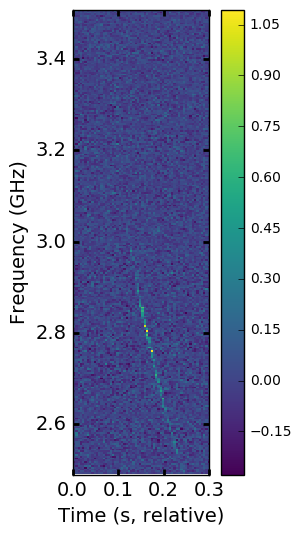
\includegraphics[width=0.18\columnwidth]{sgram_57623.png}
  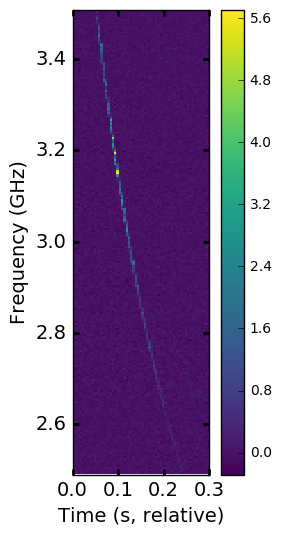
\includegraphics[width=0.18\columnwidth]{sgram_57633_scan7.png}
  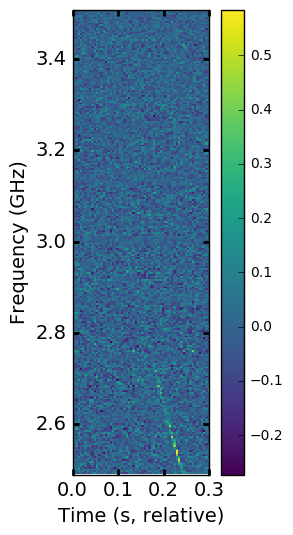
\includegraphics[width=0.18\columnwidth]{sgram_57633_scan13.png}
  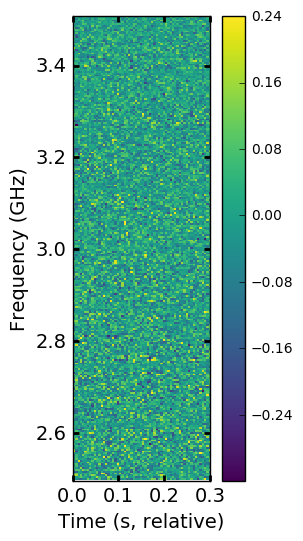
\includegraphics[width=0.18\columnwidth]{sgram_57638.png}
  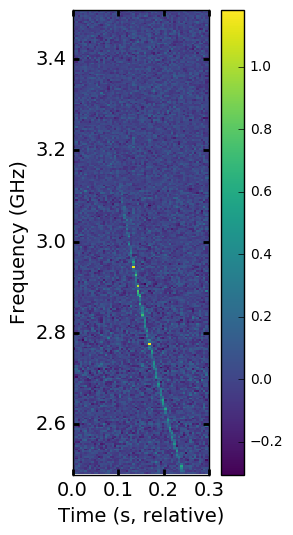
\includegraphics[width=0.18\columnwidth]{sgram_57643.png}
 \end{minipage}

 \begin{minipage}{2\columnwidth}
  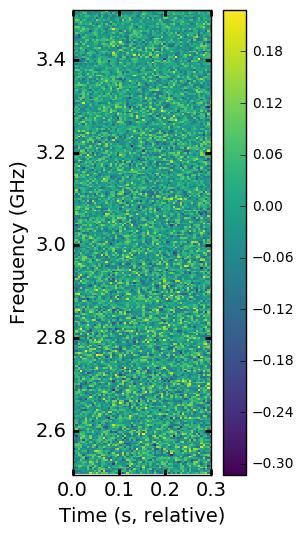
\includegraphics[width=0.18\columnwidth]{sgram_57645.png}
  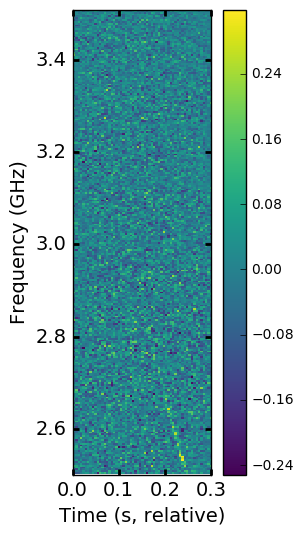
\includegraphics[width=0.18\columnwidth]{sgram_57646.png}
  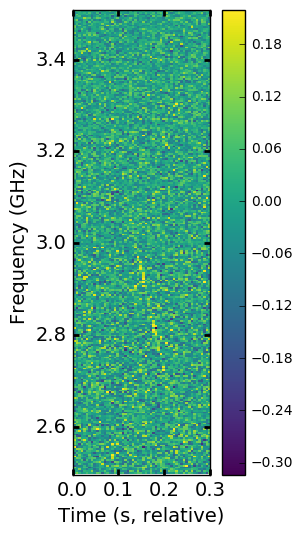
\includegraphics[width=0.18\columnwidth]{sgram_57648.png}
  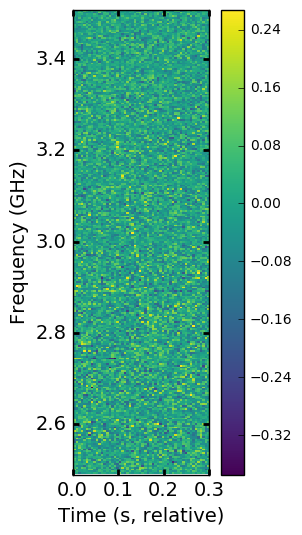
\includegraphics[width=0.18\columnwidth]{sgram_57649.png}
 \end{minipage}

 \caption{Spectrograms (time vs frequency intensity maps) for the nine VLA bursts. Starting at the top left, the correspond to bursts 57623, 57633.68, 57633.70, 57638, 57643, 57645, 57646, 57648, and 57649. Note that bursts are detected in 5~ms images generated from dedispersed visibilities.
 \label{fig:sgram}}
\end{center}
\end{figure*}


\subsubsection{Dynamic Spectra}
\label{sec:spec}
Figure \ref{fig:sgram} shows the spectrograms of all nine bursts detected by the VLA. We improved on the initial analysis presented in (CITE: LOC) by using a better calibration scheme and optimizing the detection signifnance by optimizing over a range of DM. Table \ref{tab:spec} shows the improved burst parameters using this new scheme. 

\begin{table*}
\caption{Properties of Bursts from \frb}
\centering
\begin{tabular}{lccccccc}
\hline
Date     & S$_{\rm{int}}$ & Image SNR & L$_{\rm{int}}$ & DM$_{\rm{opt}}$ & S$_{\rm{peak}}$ & Center & FWHM \\
(MJD)    & (mJy) &  & ($10^{39}$\ erg) & (pc cm$^{-3})$ & (mJy?) & (GHz) & (MHz) \\ \hline
57623    & 258 & 38 & 1.5 & 561 & 0.41             & 2.8 & 300 \\
57633.68 & 2000 & 179 & 12 & 554 & 1.90           & 3.2 & 520 \\
57633.70\tablenotemark{a} & 105 & 15 & 0.6 & 559 & $>$0.188          & $<$2.5 & $>$350 \\
57638    & 65  & 12 & 0.4 & 556 & 0.07             & 3.1 & 410 \\
57643    & 375 & 100 & 2.1 & 560 & 0.39            & 2.8 & 520 \\
57645    & 38  & 13 & 0.2 & 572 & 0.06             & 2.8 & 210 \\
57646\tablenotemark{a}    & 69  & 20 & 0.4 & 555 & $>$0.16          & $<$2.5 & $>$400 \\
57648\tablenotemark{b}    & 97 & 25 & 0.6 & 559 & 0.11 & 2.9 & 420 \\
57649    & 110 & 36 & 0.6 & 552 & 0.07             & 2.9 & 880 \\ \hline
\end{tabular}
\tablenotetext{a}{Best-fit Gaussian is not centered in 3~GHz band, so spectral parameters are limits.}
\tablenotetext{b}{Detected simultaneously with Arecibo between 1.15 and 1.73~GHz.}
\label{tab:spec}
\end{table*} 

\subsubsection{Dispersion Meausres}
The initial VLA detections were made by searching a DM grid that allowed inter-DM sensitivity losses up to roughly 10\%. For the VLA 3~GHz observing band, we estimated that trials could be separated by at most 10 pc cm$^{-3}$ \citep{2003ApJ...596.1142C}. We refined that analysis by maximizing the image SNR for DMs spaced by 1 pc cm$^{-3}$. The optimal DM values range from 552 to 572 pc cm$^{-3}$ for all bursts and from 552 to 561 pc cm$^{-3}$ for bursts with SNR$>30$. 

The uncertainty in the peak DM measurement is defined by the DM sensitivity loss curve and the significance of the burst. We tested the precision of the peak DM measuremet by simulating a burst with SNR$=30$ and measuring its detection significance as a function of DM. The simulation parameters were reproduced at the known DM with a precision of roughly 1 pc cm$^{-3}$. This suggests that the measured variation in DM for \frb is intrinsic to the bursts, rather than due to measurement uncertainty. This is consistent with the observation of intrinsic burst spectrotemporal structure that varies between bursts (CITE: WEIRD).


\subsubsection{Spectral modeling}
After finding an optimal burst DM, we extract a spectrum from the integration with peak SNR (Figure \ref{fig:spec}). After DM optimization, all bursts appear unresolved at the 5~ms time resolution of the VLA data (except maybe 57633.68, brightest burst). 

\begin{figure*}[ht]
\begin{center}
 \begin{minipage}{2\columnwidth}
  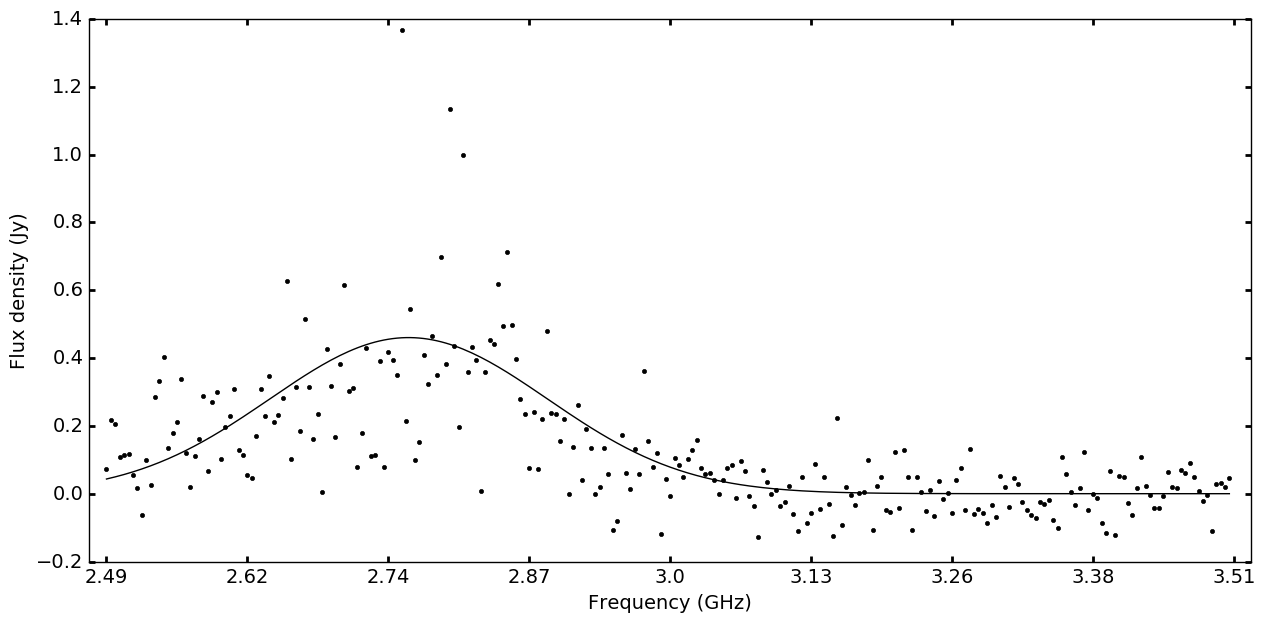
\includegraphics[width=0.3\columnwidth]{spec_57623.png}
  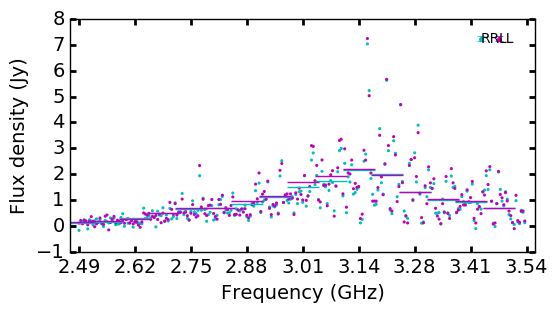
\includegraphics[width=0.3\columnwidth]{spec_57633_scan7.png}
  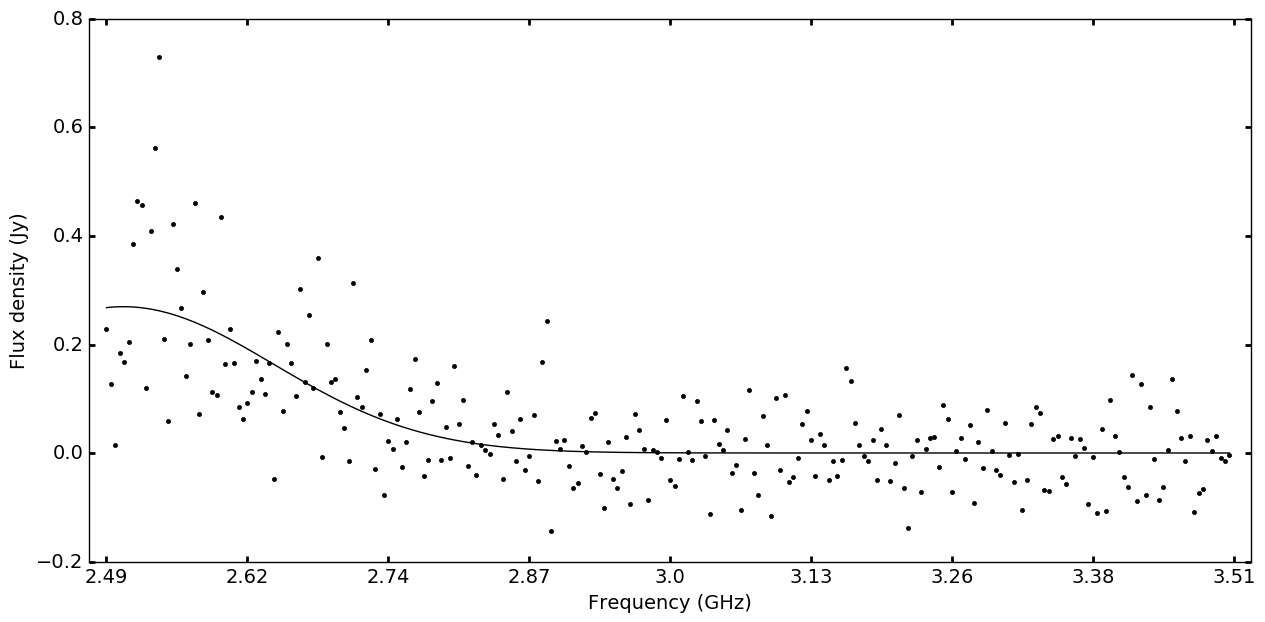
\includegraphics[width=0.3\columnwidth]{spec_57633_scan13.png}
 \end{minipage}

 \begin{minipage}{2\columnwidth}
  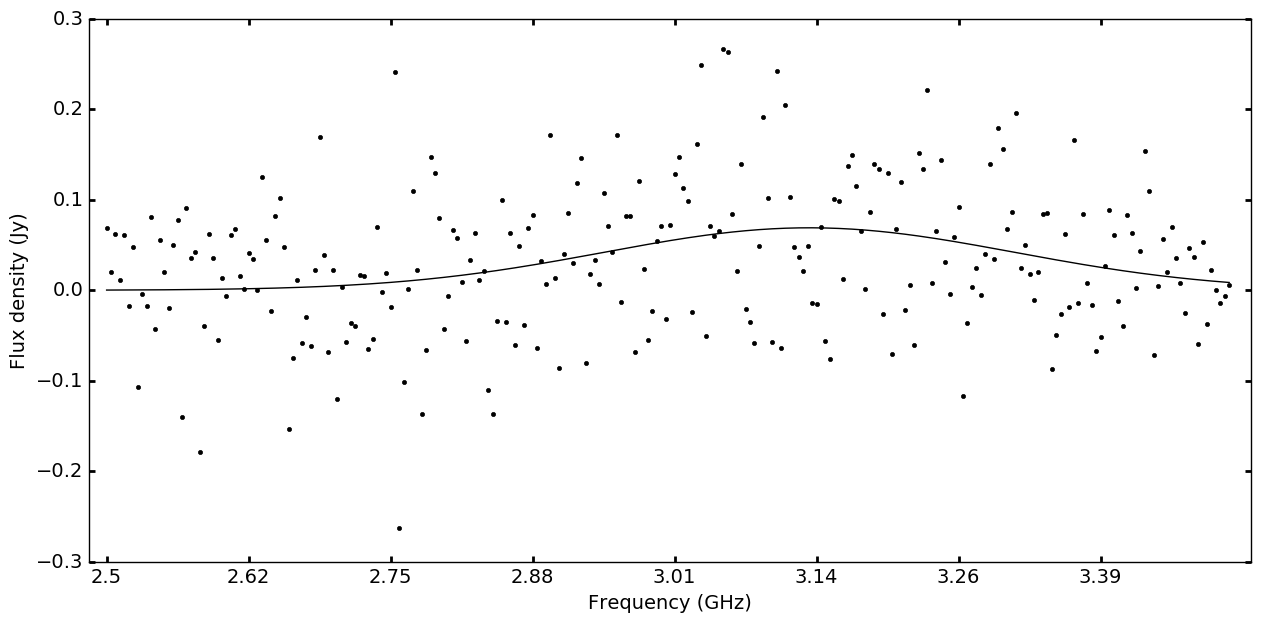
\includegraphics[width=0.3\columnwidth]{spec_57638.png}
  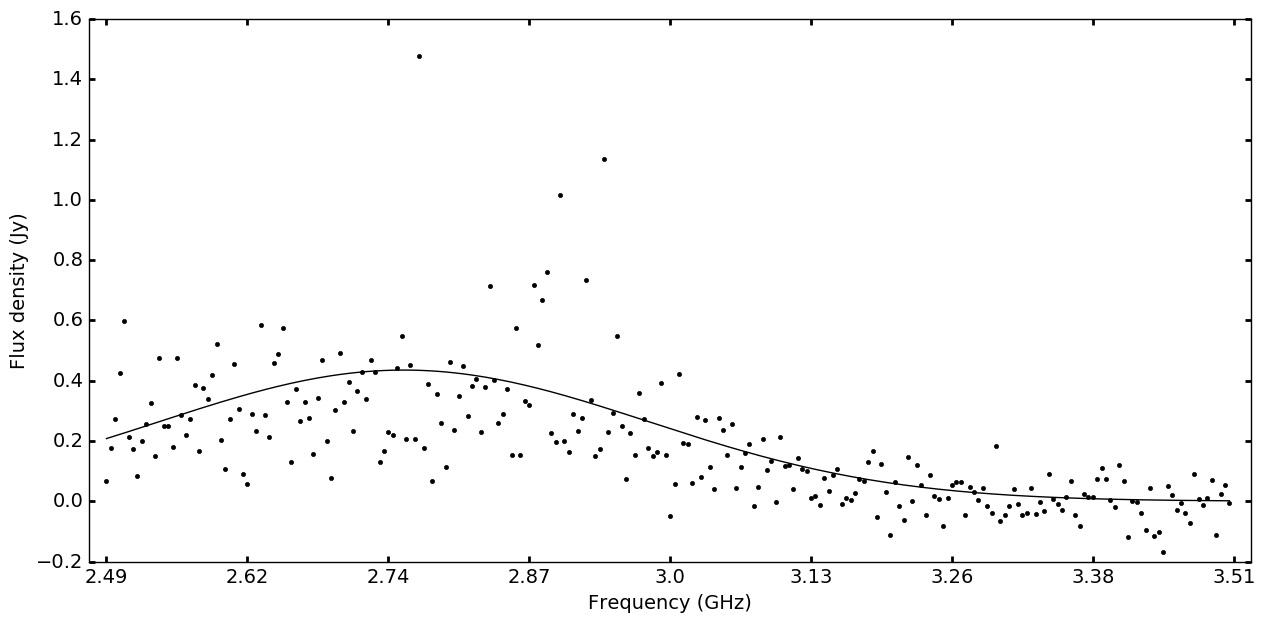
\includegraphics[width=0.3\columnwidth]{spec_57643.png}
  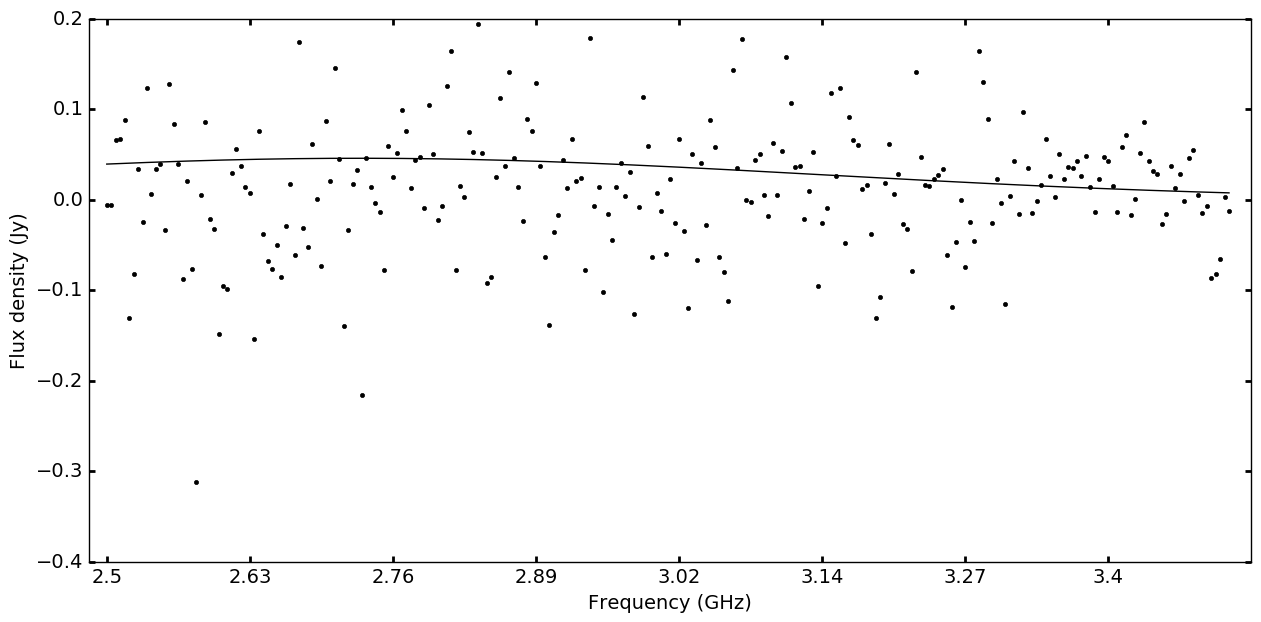
\includegraphics[width=0.3\columnwidth]{spec_57645.png}
 \end{minipage}

 \begin{minipage}{2\columnwidth}
  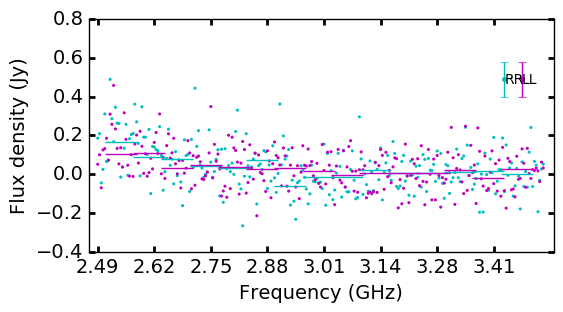
\includegraphics[width=0.3\columnwidth]{spec_57646.png}
  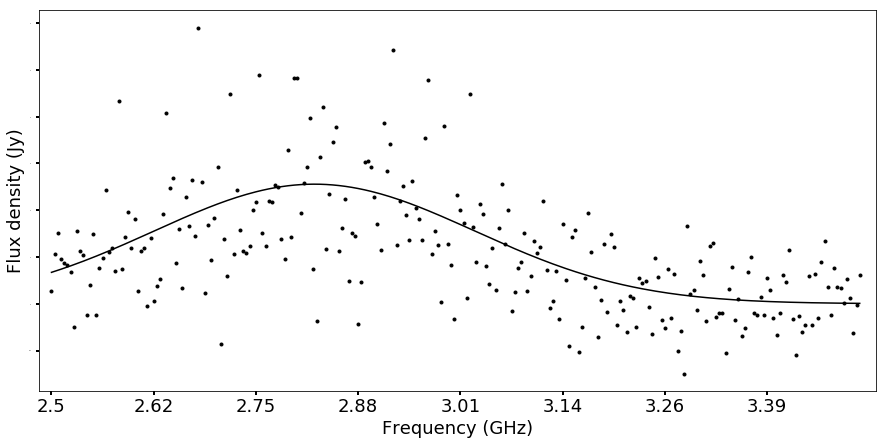
\includegraphics[width=0.3\columnwidth]{spec_57648.png}
  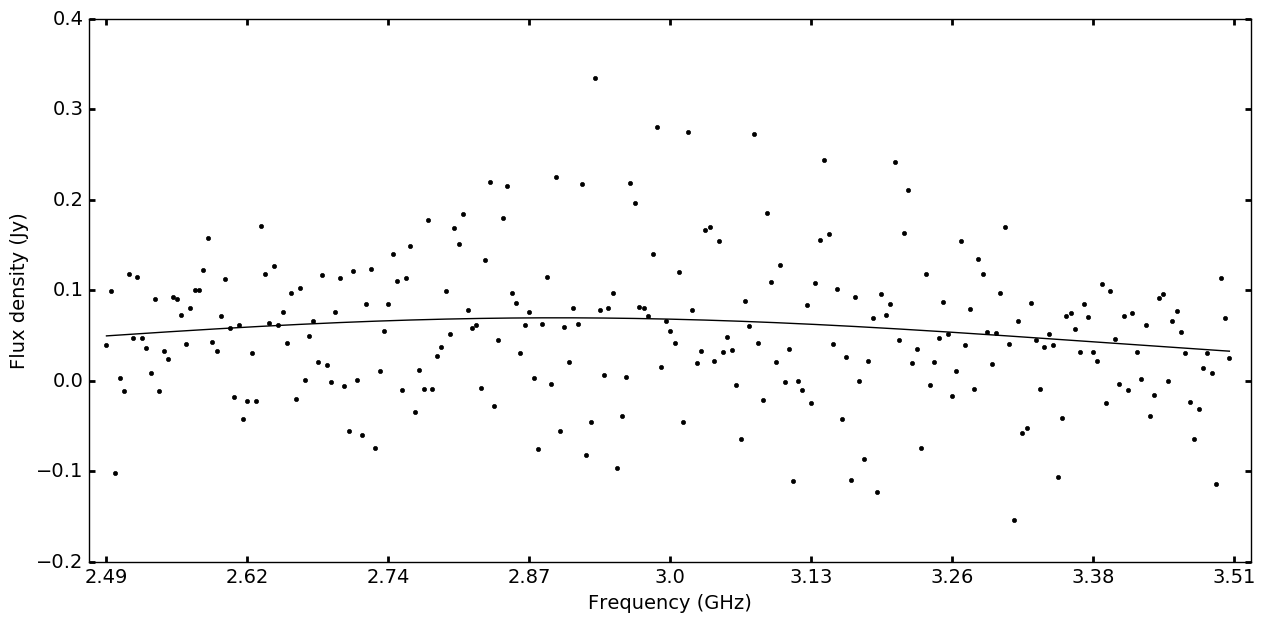
\includegraphics[width=0.3\columnwidth]{spec_57649.png}
 \end{minipage}
\caption{Spectra of nine bursts seen by the VLA from 2.5 to 3.5~GHz. Orthongonal circular polarizations (RR and LL) are plotted separately. **LABELS ALL SAME FREQ. SOME SHOULD START HIGHER FOR DROPPED CHANNELS**
\label{fig:spec}}
\end{center}
\end{figure*}

The burst spectra are generally characterized by a broad, Gaussian shape that with strong modulation between channels. We fit a Gaussian shape to each burst to estimate their characteristic width and peak flux, as summarized in Table \ref{tab:spec}. The channel-scale modulation is as high as 100\% (see \S \ref{sec:auto}) and is consistent with an exponential distribution. This introduces a strong bias to the best-fit Gaussian, but the models are reliable enough to show that the typical burst has a spectral width of 500~MHz.

All but two of the best-fit Gaussians are centered inside the 3~GHz band and most are fully contained by the 1~GHz wide band. This is consistent with previous detections of \frb by Arecibo, which showed quasi-broadband structure \citep{2016arXiv160308880S} and large variation in the implied spectral index \citep{2014ApJ...790..101S}. A detailed discussion of \frb\ burst spectra is presented in (CITE: WEIRD).

\subsubsection{Spectral Autocorrelation}
\label{sec:auto}
Autocorrelation of the burst signal (both temporal and spectral) can be used to infer both intrinsic properties and modulation due to scintillation (CITE: Cordes et al?). The VLA data have a channel resolution of 4~MHz, which is relatively coarse compared to single-dish data (e.g., CITE: WEIRD). However, diffractive scintillation observed for other FRBs \citep{} {\color{red}could/could not (Jim?)} induce structure on this scale near 3~GHz.

Figure \ref{fig:acf} shows the spectral autocorrellation for the strongest burst (MJD 57633.68). (Marginal evidence of spectral correlation on the scale of 4~MHz) {\color{red} Comment, Jim?}

\begin{figure}[htb]
\begin{center}
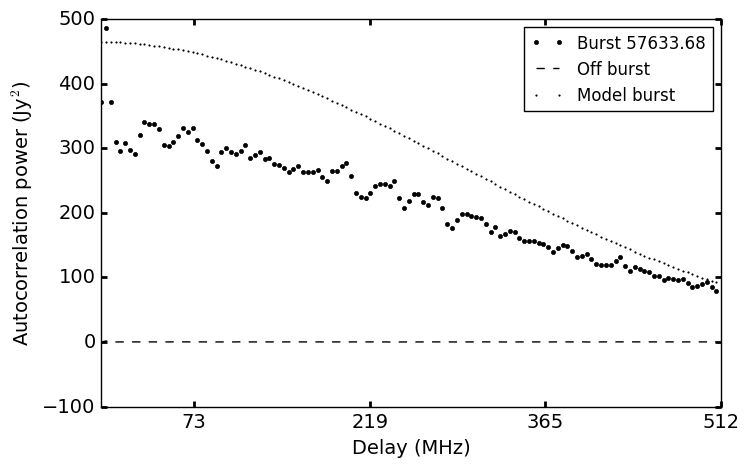
\includegraphics[width=0.9\columnwidth]{acf_57633_scan7}
\caption{The spectral autocorrelation for the burst from \frb\ at MJD 57633.68. Blue shows the autocorrelation for the burst and green shows an autocorrelation of a representative spectrum with no burst.
\label{fig:acf}}
\end{center}
\end{figure}

\subsubsection{Circular Polarization}
The VLA S-band recievers natively measure circular polarization, although for observing efficiency we chose not include polarization calibration procedures. Crude constraints on circular polarization are possible by comparing the burst intensity in right and left-hand polarized data products. The apparent circular polarization fraction ($(RR-LL)/(RR+LL)$) for the most significant bursts are all less than 3\%. FRB121102 was located 2.3 arcmin away from pointing center, where systematic effects have been measured as large as 3\% (Perley et al 2016, VLA memo). We conclude that the S-band bursts seen by the VLA have a circular polarization of less than 3\%.

\subsection{Temporal Statistics}
The VLA detected nine bursts during the month-long campaign in August--September 2016. The typical observation lasted about two hours and was sampled with a 5~ms cadence, so we used the Lomb-Scargle periodogram \citep{} to search for periodic structure over a wide range of timescales. The input "lightcurve" was mde as a one-dimensional array for all times with observations; times with a detection are set to 1 and other times are set to 0 \citep[see also]{2011MNRAS.417.1871P}. The lightcurve time resolution was set to {\color{red} 100~ms (check)} to keep the computation manageable. The 95\% confidence upper limit on periodic power is estimated by randomly selecting the 9 burst times from the same observing times. The limit is set as the 95\% highest point at each period (5th highest value in 100 simulations).

Figure \ref{fig:ls} shows the Lomb-Scargle periodogram for the bursts for periods from **xx to xx** s. No significant excess power is seen at long periods, but the periodogram shows a steady increase in power at shorter periods. The periodogram exceeds the 95\% power limit for periods from xx to xx s (**limited by binning time?**). This is consistent with the idea that the bursts imperfectly trace an underlying rotational period, as has been observed from many classes of neutron star. Examples include magnetars, which typically have wide pulse phase windows \citep{}, pulsars with glitches that change their periods \citep{}, and {\color{red} Maura? also refs for previous points would be welcome}. However, we can show with simulations that nine bursts drawn from a simple rotational would produce a strong, narrow peak in \ref{fig:ls}.

Assuming periods with power peaks, we find clusters of bursts with same rotational phase...

\begin{figure}[htb]
\begin{center}
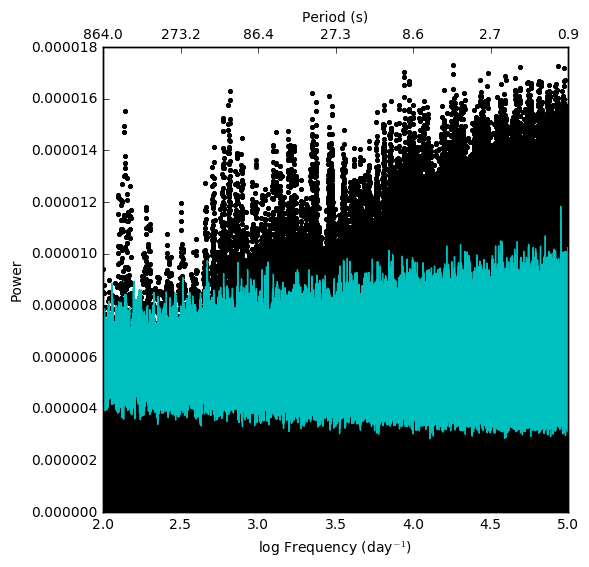
\includegraphics[width=0.9\columnwidth]{lombscargle}
\caption{Dots show the Lomb-Scargle periodogram of burst arrival times for \frb. The solid line show the 95\% confidence upper limit on the power expected from bursts with random arrival times. (**New version being compiled**)
\label{fig:ls}}
\end{center}
\end{figure}

Burst detections were made very inhomogenously through the larger (63 hours) observing campaign of FRB 121102. In the first 30 hours of observing at S-band no bursts were detected, while nine bursts were detected in the last 27 hours of S-band observing. The data quality is high and RFI did not significantly impact sensitivity, so the inhomogeneous burst distribution shows that the burst detection probability was not stationary. Assuming that the burst detection probability follows a Poisson distribution, the nondetection in the first half of S-band limits the FRB rate to $\rm{R}<0.1$ hour$^{-1}$ (95\% confidence limit). The mean detection rate for the last part of the campaign was $\rm{R}=0.3$ hour$^{-1}$.

Moreover, there is weak evidence that the \frb\ burst rate changes during the last part of the campaign. We modeled the event detection probability as a Poisson probability with a rate parameter that evolves linearly with time relative to first burst detection. We directly sampled the model by calculating the joint probability $\prod_{i} P_i$, where $P_i$ follows a Poisson probability with rate $\lambda = a + b * (\rm{MJD}_i - 57623)$. Figure \ref{fig:rate} shows that the probability distribution excludes a constant rate with $\sim$85\% confidence. This weak constraint is consistent with the broader trend seen by the VLA and Arecibo (CITE: WEIRD?).

\begin{figure}[htb]
\begin{center}
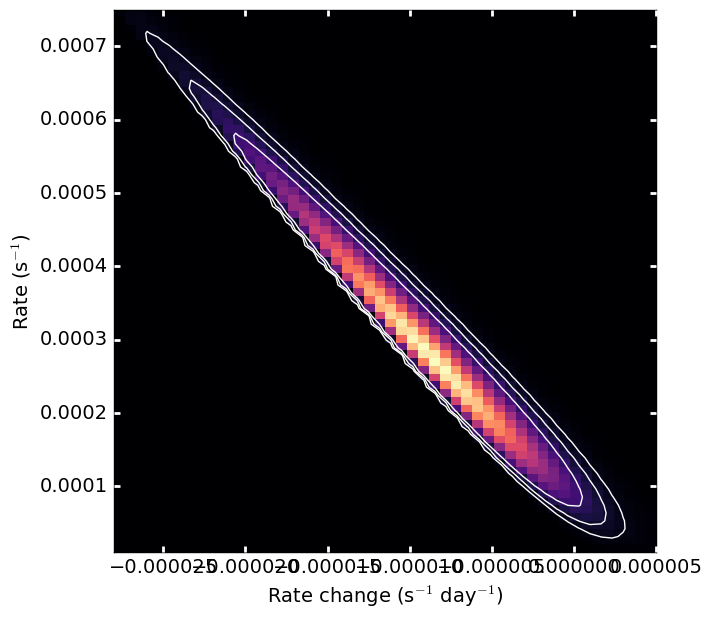
\includegraphics[width=0.9\columnwidth]{event_rate_contours}
\caption{Color scale and contours show the relative probability for a time-evolving Poisson detection probability for \frb. Contours show the 50, 90, and 95\% confidence contours on the rate $a$\ (bursts s$^{-1}$) and rate change $b$\ (bursts s$^{-1}$ day$^{-1}$) during the August--September 2016 campaign in which bursts were detected.
\label{fig:rate}}
\end{center}
\end{figure}

\subsection{Brightness Distribution}
Knowing the burst distance, we calculate their mean luminosity across a single 5~ms integration and the 1~GHz bandwidth (Table \ref{tab:spec}). The VLA has also shown for the first time that most bursts are contained within the 3~GHz band. That means that the mean S-band flux density can be converted to a luminosity in units of ergs with no assumptions about its spectral properties.

With a uniform sample of burst luminosities, we can use their distribution to infer more general properties for \frb. Figure \ref{fig:lumd} shows the luminosity distribution of the VLA bursts with a best-fit powerlaw model. Fitting a powerlaw model to the cumulative luminosity distribution gives an index of --0.5. The flatness of the distribution is also clear from range of significance of the nine bursts (12 to 179$\sigma$). All bursts are much brighter than the sensitivity limit (weakest is $\sim10\sigma$), so the distribution is not affected by a completeness limit.

\begin{figure}[htb]
\begin{center}
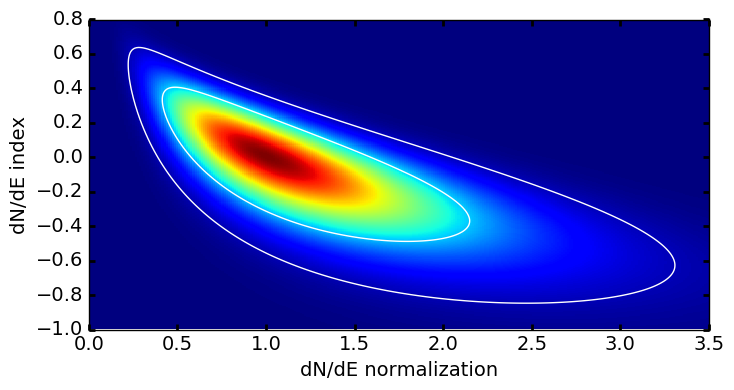
\includegraphics[width=0.9\columnwidth]{luminosity_disn}
\caption{Cumulative luminosity distribution and best-fit powerlaw model for the nine VLA bursts from \frb.
\label{fig:lumd}}
\end{center}
\end{figure}

\section{discussion}

\subsection{Luminosity Distribution}
Doubts were cast on the first FRB detection (``Lorimer burst'') due to its unusually high brightness. The lack of lower-significance detections suggested that this burst was unlikely to be part of any astrophysical population. With more detections, it has become clear that the FRB population has a relatively flat flux distribution \citep{2016ApJ...830...75V, 2016arXiv161100458L}. This fact was demonstrated with yet another detection of an extremely bright FRB \citep{2016arXiv161105758R}.

Discuss comparison FRB 121102 luminosity distribution to that of FRB population...

Imagine physical log N/log S with cut-offs and scattering can bias the intrinsic into the observed distribution (Macquart and Johnston)...

Simulate cosmic volume uniformly filled with \frb...


\subsection{Repetition}
Discussion of ``red spectrum'' and \citet{2016MNRAS.458L..89C}. Bursts predict bursts therefore repetition constraints of other FRBs are likely weaker than claimed...

Constraints on repetition assuming "red spectrum" for whole population. Simulation using observed burst temporal statistics...

Intrinsic versus refractive scintillation...

Fewer FRBs out there...

\subsection{Emission Physics and Burst Energetics}

% from first paper
For a nominal Gpc distance $D$ corresponding to redshifts $z\lesssim 0.3$, the received fluence $A_{\nu}$ from each burst implies  a burst energy
$$E_{\rm burst} = 4\pi D^2 (\delta\Omega/4\pi) A_{\nu} \Delta\nu
\approx 10^{38}\, {\rm erg}\,(\delta\Omega/4\pi) D_{\rm Gpc}^2  (A_{\nu} / 0.1\ {\rm Jy\ ms}) \Delta\nu_{\rm GHz}.$$
The unknown  emission solid angle $\delta\Omega$
could be very small due to relativistic beaming, and together with a distance possibly much smaller than 1~Gpc, could reduce the energy requirement significantly.  However, the {\it total} energy emitted could be larger depending on the duration of the emission in the source frame and other model-dependent details.
Either way, the burst energies from \frb\ are not inconsistent with those that might be expected from the magnetosphere of a compact object\cite{2016MNRAS.457..232C}.



\subsection{Observing Strategies}

Repetition implies that targeting known FRBs is optimal.

Repetition and shallow luminosity distribution show that shallow and wide is the best way to blindly find FRBs.

Given that bursts have $<1$~GHz-scale spectra, wide bandwidths improve odds of detection.

\section{Conclusions}

 % include timeline and science scope for new localizations? realfast plug and reference cosmology papers, contingency on DMhost, etc.

\bibliographystyle{apj}

\section*{Acknowledgements}
We thank ...
This project was supported by the University of California Office of the President under Lab Fees Research Program Award 237863. The National Radio Astronomy Observatory is a facility of the National Science Foundation operated under cooperative agreement by Associated Universities, Inc.. This research made use of Astropy, a community-developed core Python package for Astronomy (Astropy Collaboration, 2013).

\bibliography{fasttrants.bib}

%\begin{figure}[htb]
%\begin{center}
%\includegraphics[width=0.9\columnwidth]{}
%\caption{
%\label{fig:name}}
%\end{center}
%\end{figure}

%\begin{table}
%\caption{Caption}
%\footnotesize
%\centering
%\begin{tabular}{l|cc|cc|c}
%\hline
%Field       & RA          & Dec   & Lon. & Lat.     & Time \\
%            & \multicolumn{2}{|c|}{(J2000)}  & \multicolumn{2}{|c|}{(Galactic; deg)} & (hrs) \\ \hline
%RA02        & 2:27:53  &  +9:13:24 & 159.0 & --46.8    & 26.25 \\
%PSR J2248-0101 & 22:48:27 & --1:1:48 & 69.3 & --50.6 & 6.5 \\ \hline
%\end{tabular}
%\label{fields}
%\end{table} 

\end{document}

